\begin{figure}
\centering
\newcommand{\wmg}{0.5\columnwidth}  % width maunu growth
\newcommand{\hmg}{0.5\columnwidth}             % height maunu growth
\begin{tabular}{c}
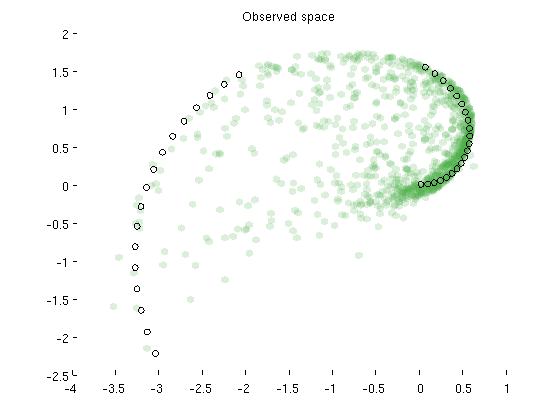
\includegraphics[width=\wmg,height=\hmg]{figures/first_demo_nocensor} 
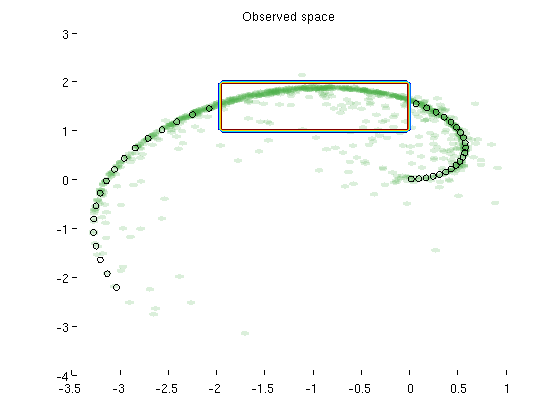
\includegraphics[width=\wmg,height=\hmg]{figures/second_demo_censor}
\end{tabular}
\caption{Modeling a truncated dataset.  Left:  Naively fitting a density manifold to the data.  Right:  When truncation is modeled explicitly, the model is not penalized for placing mass in censored regions, even though there is no mass there.}
\label{fig:synthetic}
\end{figure}

